\section{Introduction}\label{sec:intro}
Virtual Reality (VR) technology is thriving in various business sectors,
including computer games, tourism industry, real estates, and occupational trainings. 
The VR scenes can either be generated with computer graphics or captured from nature scenes, 
which provide omnidirectional, a.k.a. 360{\degree}, viewing experience of virtual worlds. 
It is estimated that the global VR market size will reach 26.89 billion USD by 2022, 
with an annual growth rate of 54\% from 2017 to 2022~ \cite{VR_market}.
As VR technology becomes more and more mature, 
researchers start to study its Quality of Experience (QoE) in order to deliver higher-quality scenes for better user experience.

\begin{figure}[tbh]
	\begin{center}
		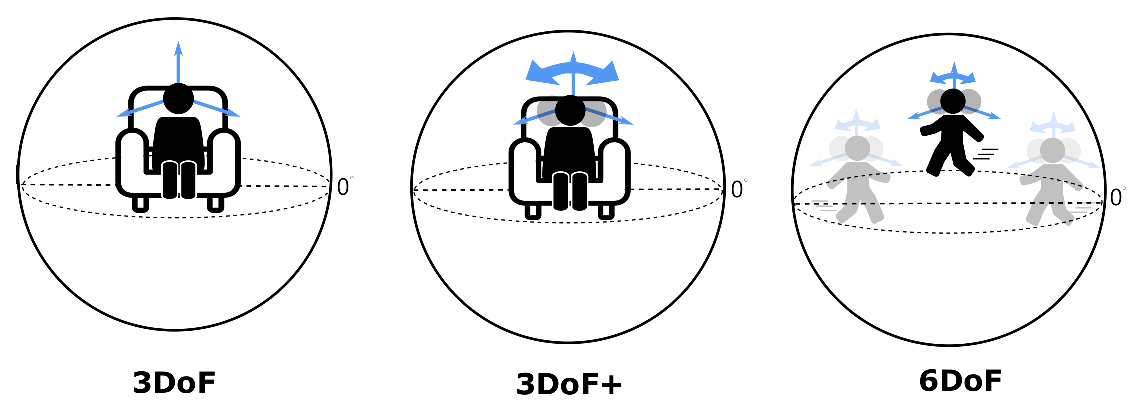
\includegraphics[width=.5\textwidth]{fig/vr_phase}
		\caption{Three phases of VR technology development. The spheres represent the virtual worlds.}
		\label{fig:vr_phase}
	\end{center}
\end{figure}

% Difference between 3DoF+ and 6DoF
One key factor affecting the QoE of VR technology is the way users interact with the virtual worlds. 
MPEG-I group has defined three development phases of the VR technology: 3 Degree-of-Freedom (3DoF), 3DoF+, and 6DoF, which are illustrated 
in Fig.~\ref{fig:vr_phase}.
3DoF VR technology allows users to rotate their heads in three dimensions, which are represented by yaw $\psi$, pitch $\theta$, and roll $\phi$. 
However, with 3DoF VR, when users move their heads or stand up and walk, their position changes do {\em not} affect the views rendered in the 
Head-Mounted Displays (HMDs).
To overcome this limitation, 3DoF+ VR is proposed to support {\em limited} movements.
Namely, users can slightly move their heads to a certain extent when sitting on fixed chairs. 
6DoF VR further enables users to freely move, e.g., walk, in virtual worlds.
Users can not only rotate their heads in three dimensions but also move in the three additional dimensions, which are $x$, $y$, $z$ coordinates. 

A naive way to achieve 3DoF+ and 6DoF is to capture multiple 360$^{\circ}$ videos at different positions~\cite{CSSF18,PZWL+19}, 
and only allow the HMD users to 
switch among these discrete positions in the scenes.
We target more general 3DoF+ and 6DoF VR, where users can freely move in among the discrete positions.
We refer to the streaming systems that support such 3DoF+ and 6DoF VR as {\em immersive video streaming} throughout this proposal.

Achieving real immersive video streaming is not an easy task, because there are many challenges need to be overcome:
\begin{itemize}
	\item {Different Data Representations: } Various data types can be used to store the information of immersive video, e.g.,
	2D texture and depth image, light field, 3D point cloud, 3D mesh. Each of them has pros, cons, and usage scenarios, which hav not been comprehensively studied.
	\item {Strict Network Condition Requirements: } The data representations of immersive video have a huge data size. 
	They need a lot of bandwidth to be streamed, while the realtime ness needs to be maintained. 
	Take light field video as an example, streaming it consumes bandwidth in the range between 
	200 Gb/s and 1 Tb/s \cite{CVRW+20}, which is much higher than the available bandwidth we consume today.
	Moreover, the interactive applications, e.g., 6DoF VR games and holographic conferences, need low latency to realize real-time communications.
	This inturn makes the network condition requirements more strict.
	\item {User Experiences: } User experience is the quality that perceived by  users. 
	It is an important performance metric for multimedia applications.
	However, the user experience of immersive videos is still not explored,
	and the challenges of measuring user experience include but not limited: 
	(i) too many parameters may affect the user experience in immersive video streaming.
	and (ii) it's hard to build a immersive video streaming testbed.
	% Estimating the user experience can help us find the pattern of user habit. 
	% We can reduce the video quality of user not sensitive part to save the network and computing resources.
	
\end{itemize}
% To achieve real immersive video streaming, there are some candidate of data representations:
% XXX todo intro. these data type XXX 
% \begin{itemize}
% 	\item {\bf Depth Image Based Rendering (DIBR): }
% 	\item {\bf Light Field: }
% 	\item {\bf 3D Point Cloud: }
% 	\item {\bf 3D Mesh: }
% \end{itemize}

In this research proposal, we propose three research directions to address the three challenges:
(i) {\em Data Representations} 
(ii) {\em Optimal Streaming} 
(iii) {\em Quality of Experience}. 
We introduce them in details below.
% In our first work \cite{mm20_tr},
% we use Test Model for Immersive Video (TMIV)~\cite{mpeg_N18470,mpeg_N18577,mpeg_N18795}, 
% which is a DIBR codec for immersive video streaming from MPEG, to optimize the immersive video streaming.
% we develop algorithms to solve the configuration optimization problem based on deep learning, particularly the Neural Network (NN) approaches.
% The two proposed algorithms are:
% a Convolutional Neural Network (CNN) based algorithm and a Deep Reinforcement Learning (DRL) based algorithm
% \footnote{We refer to them as CNN and DRL algorithms for short in the rest of this paper.}.
% Our CNN algorithm benefits from: (i) automatic extracting latent features and 
% (ii) inferencing the prediction rapidly and directly according to the input, which allows the configuration optimizer to 
% adapt to various video scenes and dynamic camera parameters.
% Our DRL algorithm systematically builds an {\em agent} that can adapt to dynamic {\em environments}~\cite{SB18,PZWL+19,HZZS18,CIZI+19}.
% The trained agent learns how to quickly search through a large space for optimal configurations. 
% The two proposed algorithms are
% trained to adaptively find the optimal configurations given the diverse video content, HMD user behaviors, and user-specified utility functions.

% Our paper makes the following contributions:
% \begin{itemize}
% \item We propose the first NN-based algorithms\footnote{We also refer to NN-based algorithms as NN algorithms for brevity.} designed for configuration
% optimization of TMIV. Our solution approach can be readily adapted to other
% usage scenarios and immersive video systems.
% \item We conduct extensive experiments with real datasets to evaluate the
% performance of our algorithms. Our objective experiments show that the proposed
% algorithms consume less resources compared to the default and optimal TMIV
% configurations.
% \item We conduct a user study to subjectively evaluate the synthesized view
% quality among configurations generated by different algorithms.
% A detailed analysis shows
% that the difference of the synthesized view quality is insignificant among them.
% \end{itemize}
% We submitted our paper to ACM Multimedia Conference 2020.
